\documentclass{article} 
\usepackage[utf8]{inputenc}
\usepackage{mathtools, amsmath,graphicx, fontawesome5, titlesec}
\usepackage[most]{tcolorbox}
\usepackage[scale=.95,type1]{cabin}
\usepackage[framemethod=tikz]{mdframed}


\usepackage[legalpaper,margin=1in]{geometry}

\setlength{\parindent}{10pt}
\setlength{\parskip}{1em}
\renewcommand{\baselinestretch}{1.2}

\title{}
\date{}
\author{}
\usepackage{tabularray}

\newcounter{Def}[section]
\newenvironment{Def}[1][]{%
  \ifstrempty{#1}%
  {\mdfsetup{%
    frametitle={%
      \tikz[baseline=(current bounding box.east),outer sep=0pt]
      \node[line width=1pt,anchor=east,rectangle,draw=blue!20,fill=white]
    {\strut \color{black}{Definition}~};}}
  }%
  {\mdfsetup{%
    frametitle={%
      \tikz[baseline=(current bounding box.east),outer sep=0pt]
      \node[line width=1pt,anchor=east,rectangle,draw=blue!20,fill=white]
    {\strut \color{black}{Definition}~:~\color{blue4}{#1}};}}%
  }%
  \mdfsetup{innertopmargin=2pt,linecolor=blue!20,%
            linewidth=1pt,topline=true,%
            frametitleaboveskip=\dimexpr-\ht\strutbox\relax,}
  \begin{mdframed}[]\relax%
  }{\end{mdframed}}
%{\fontfamily{cmtt}\selectfont }
\titleformat{\section}
  {\fontfamily{lmss}\selectfont\LARGE\bfseries\color{black}}
  {\thesection}{1em}{}
\begin{document}
\section{The {\fontfamily{lmtt}\selectfont Foldable} class}
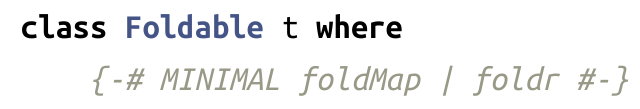
\includegraphics[width = 6 cm]{./Foldable.png}

  {\fontfamily{lmtt}\selectfont MINIMAL.}  {\fontfamily{lmtt}\selectfont foldMap} and {\fontfamily{lmtt}\selectfont foldr} can be implemented in terms of the other, and other operations of the typeclass can be implemented in terms of either. Define 1 and get a working instance! Some methods have default implementation.

  % 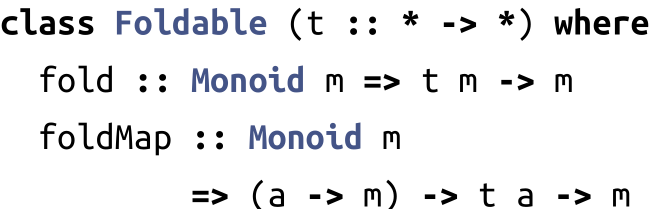
\includegraphics[width = 5.7 cm]{./classFold.png}
  
  The fact that the numbers in our list have other possible monoid is not relevant once we've specified which operation to use.

  With only one value, no need {\fontfamily{lmtt}\selectfont Monoid} instance.
\end{document}
